\tikzstyle{vtx}=[draw,circle,fill,minimum width=1pt]

\tikzstyle{ed}=[color=blue]

\begin{figure}[h!]
    \centering
    \scalebox{.8}{

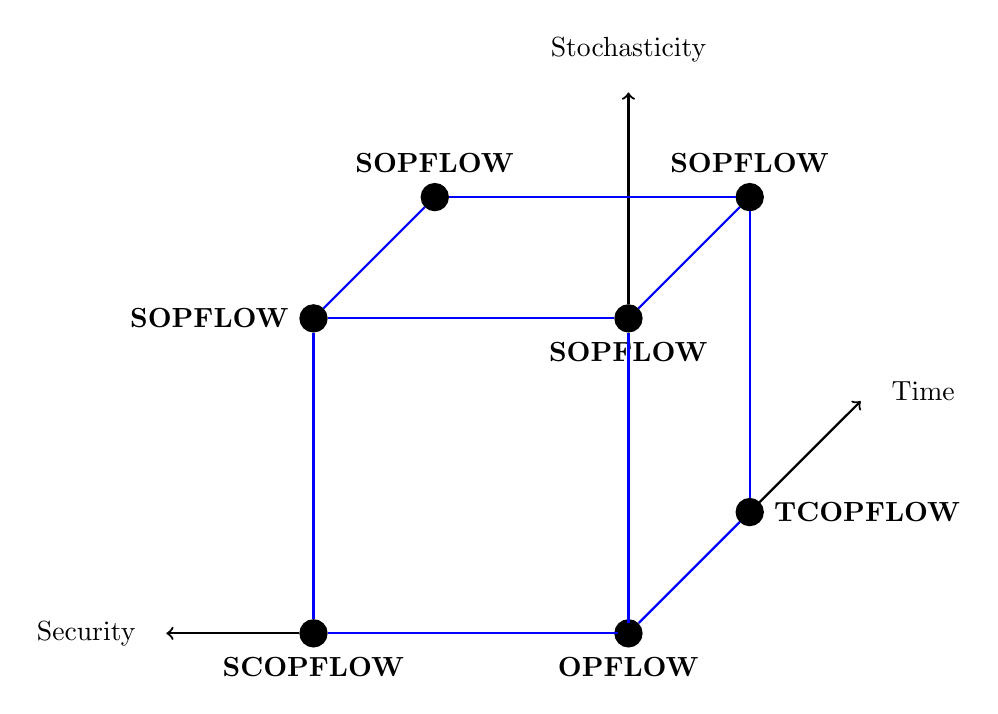
\begin{tikzpicture}[auto, thick]
   \node (o) at (0,0,0) {};
   \node[label=left:{Security}] (x) at (-6,0,0) {}; 
   \node[label=above:{Stochasticity}] (y) at (0,7,0) {}; 
   \node[label=right:{Time}] (z) at (0,0,-8) {}; 
 % \node[time,label=below:$t_0$] (t0) at (0,0) {};
 % \node[time,label=below:$t_1$] (t1) at (2,0) {};
 % \node[time,label=below:$t_2$] (t2) at (4,0) {};
 % \node[time,label=below:$t_3$] (t3) at (6,0) {};
  
  \node[vtx,label=below:\textbf{OPFLOW}] (opflow) at (0,0,0) {};
  \node[vtx,label=right:\textbf{TCOPFLOW}] (tcopflow) at (0,0,-4) {};
  \node[vtx,label=below:\textbf{SCOPFLOW}] (scopflow) at (-4,0,0) {};
  \node[vtx,label=below:\textbf{SOPFLOW}] (sopflow) at (0,4,0) {};
  

  \node[vtx,label=above:\textbf{SOPFLOW}] (b) at (0,4,-4) {};
  \node[vtx,label=left:\textbf{SOPFLOW}] (c) at (-4,4,0) {};
  \node[vtx,label=above:\textbf{SOPFLOW}] (d) at (-4,4,-4) {};
  
  \path (scopflow) edge [->,thick] (x);
  \path (sopflow) edge [->,thick] (y);
  \path (tcopflow) edge [->,thick] (z);
  
  \path (sopflow) edge [ed] (b);
  \path (sopflow) edge [ed] (c);
  \path (b) edge [ed] (d);
  \path (c) edge [ed] (d);
  
  \path (scopflow) edge [ed] (c);
  \path (tcopflow) edge [ed] (b);
  \path (o) edge [ed] (tcopflow);
  \path (o) edge [ed] (scopflow);
  \path (o) edge [ed] (sopflow);
 % \path (t0) edge (t1);
 % \path (t1) edge (t2);
 % \path (t2) edge (t3);


\end{tikzpicture}}
\caption{\exago provides applications along the dimensions of security (contingencies), time, and stochasticity. The label vertices denote different \exago applications available.}
\label{fig:intro_fig}
    
\end{figure}